\documentclass[tikz,border=8pt]{standalone}
\usepackage{amsmath}\usepackage{pgfplots}\pgfplotsset{compat=1.18}\usetikzlibrary{arrows.meta}
\definecolor{ink}{HTML}{334155}\definecolor{blue}{HTML}{6366F1}\definecolor{green}{HTML}{059669}\definecolor{orange}{HTML}{EA580C}
\begin{document}
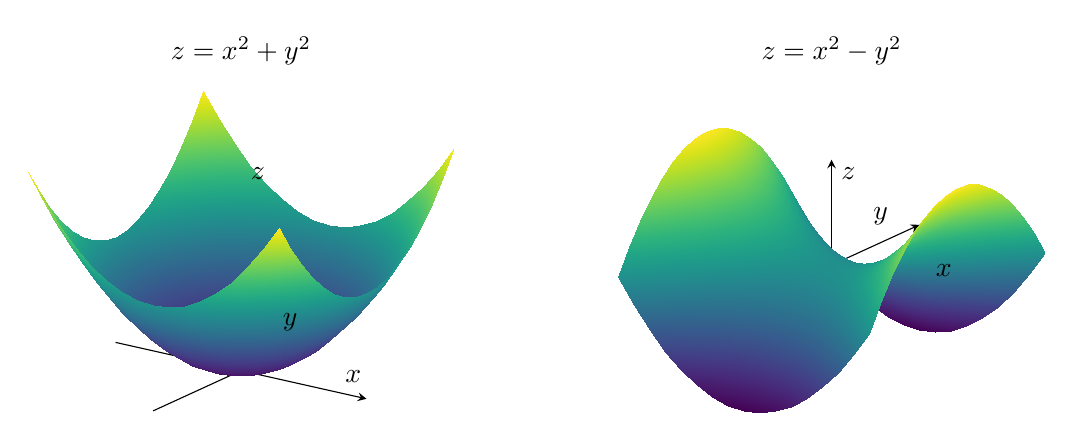
\begin{tikzpicture}
\begin{axis}[width=7cm,height=6cm,view={35}{25},axis lines=center,xlabel=$x$,ylabel=$y$,zlabel=$z$,ticks=none,title={$z=x^2+y^2$}]
\addplot3[surf,shader=interp,domain=-1:1,y domain=-1:1,samples=17,colormap/viridis]{x^2+y^2};\end{axis}
\begin{axis}[at={(7.5cm,0)},anchor=south west,width=7cm,height=6cm,view={35}{25},axis lines=center,xlabel=$x$,ylabel=$y$,zlabel=$z$,ticks=none,title={$z=x^2-y^2$}]
\addplot3[surf,shader=interp,domain=-1:1,y domain=-1:1,samples=17,colormap/viridis]{x^2-y^2};\end{axis}\end{tikzpicture}
\end{document}
